\documentclass[portrait,final,a0paper,]{baposter}

\usepackage[francais]{babel}
\usepackage[utf8]{inputenc}
\usepackage[T1]{fontenc}

\usepackage{calc}
\usepackage{graphicx}
\usepackage{amsmath}
\usepackage{amssymb}
\usepackage{relsize}
\usepackage{multirow}
\usepackage{rotating}
\usepackage{bm}
\usepackage{enumitem}
\usepackage{url}
\usepackage{booktabs}
%\usepackage{multicol}
\usepackage{xcolor}
\usetikzlibrary{calc}

\usepackage{tabularx}


%\usepackage{times}
\usepackage{helvet}
%\usepackage{bookman}
%\usepackage{palatino}
\renewcommand*{\familydefault}{\sfdefault}

\newcommand{\captionfont}{\footnotesize}

\graphicspath{{images/}}

\setlength{\columnsep}{1.5em}
\setlength{\columnseprule}{0mm}

\newcommand{\marktikz}[1]{ \tikz[remember picture,overlay]\node (#1) {};}
\renewcommand{\baselinestretch}{1.05} 

%%%%%%%%%%%%%%%%%%%%%%%%%%%%%%%%%%%%%%%%%%%%%%%%%%%%%%%%%%%%%%%%%%%%%%%%%%%%%%%%
% Save space in lists. Use this after the opening of the list
%%%%%%%%%%%%%%%%%%%%%%%%%%%%%%%%%%%%%%%%%%%%%%%%%%%%%%%%%%%%%%%%%%%%%%%%%%%%%%%%
\newcommand{\compresslist}{%
\setlength{\itemsep}{1pt}%
\setlength{\parskip}{0pt}%
\setlength{\parsep}{0pt}%
}

\newcommand{\diag}[1]{\lceil#1\rfloor}
\newcommand*\circled[1]{\tikz[baseline=(char.base)]{
            \node[shape=circle,draw,inner sep=2pt,color=main,fill=main!10, line width=1pt] (char) {#1};}}

%%%%%%%%%%%%%%%%%%%%%%%%%%%%%%%%%%%%%%%%%%%%%%%%%%%%%%%%%%%%%%%%%%%%%%%%%%%%%%
%%% Begin of Document
%%%%%%%%%%%%%%%%%%%%%%%%%%%%%%%%%%%%%%%%%%%%%%%%%%%%%%%%%%%%%%%%%%%%%%%%%%%%%%

\begin{document}

%%%%%%%%%%%%%%%%%%%%%%%%%%%%%%%%%%%%%%%%%%%%%%%%%%%%%%%%%%%%%%%%%%%%%%%%%%%%%%
%%% Here starts the poster
%%%---------------------------------------------------------------------------
%%% Format it to your taste with the options
%%%%%%%%%%%%%%%%%%%%%%%%%%%%%%%%%%%%%%%%%%%%%%%%%%%%%%%%%%%%%%%%%%%%%%%%%%%%%%
% Define some colors


\definecolor{green}{rgb}{0.32,0.67,0.39}
%\definecolor{main}{rgb}{0 0.627 0.588} %canard
\definecolor{main}{rgb}{0 0.439  0.753} %bleu %0 112 192
\definecolor{rouge}{rgb}{1 0.270 0 } %255 69 0
\definecolor{jaune}{rgb}{1 0.745 0} %255 190 0
\definecolor{vert}{rgb}{0.573 0.792 0.209} %146 202 74
%\hyphenation{resolution occlusions}
%%
\begin{poster}%
  % Poster Options
  {
  % Show grid to help with alignment
  grid=false,
  % Column
  columns=6,
  colspacing=1em,
  % Color style
  background=plain,%%shadetb,
  bgColorOne=gray!12,%lightestgreen!80,
  bgColorTwo=white,
  borderColor=white,%darkgreen,
  headerColorOne=white,%darkgreen,
  %headerColorTwo=lightgreen,
  headerFontColor=main,%white,
  boxColorOne=white,%lightestgreen,
  %boxColorTwo=lightgreen,
  % Format of textbox
  textborder=roundedleft,%faded,
  % Format of text header
  eyecatcher=false,
  headerborder=closed,
  headerheight=0.087\textheight,
  %textfont=\sc,% An example of changing the text font
  headershape=roundedright,
  headershade=plain,%shadelr,
  headerfont=\Large\bfseries,%\textsc, %Sans Serif
  textfont={\setlength{\parindent}{1.5em}},
  boxshade=plain,
  linewidth=2pt
  }
  % Eye Catcher
  {  }
  % Title
 {
%\begin{tikzpicture}[overlay, remember picture, inner sep=0pt, outer sep=0pt]
%  %\fill [white] ([yshift=-3cm]current page.north west) rectangle (current page.north east);
%\end{tikzpicture}
%\begin{minipage}{\linewidth}
%	\vspace{0.5cm}
%	\includegraphics[height=1cm]{logo/LABEX_CELYA.jpg} \hfill \includegraphics[height=1cm]{logo/logo_lmfa.pdf} \hfill \includegraphics[height=1cm]{logo/LVA_compact_couleur_transparent.png} \hfill   \includegraphics[trim={0 3cm 0 3cm},clip=true,height=1cm]{logo/logo_ADAPT.png}\\
%\end{minipage} 
\vspace{0.4cm}\textcolor{main}{\textbf{Débruitage de la matrice interspectrale pour l'étude des sources aéroacoustiques}}}
  % Authors
  { ~\\ \textit{A. Dinsenmeyer}\textsuperscript{1,2}, Q. Leclère\textsuperscript{1}, J. Antoni\textsuperscript{1}, E. Julliard\hspace{0.1ex}\textsuperscript{3}}
  % University logo
  {  }
  
 
%%%%%%%%%%%%%%%%%%%%%%%%%%%%%%%%%%%%%%%%%%%%%%%%%%%%%%%%%%%%%%%%%%%%%%%%%%%%%%
%%% Now define the boxes that make up the poster
%%%---------------------------------------------------------------------------
%%% Each box has a name and can be placed absolutely or relatively.
%%% The only inconvenience is that you can only specify a relative position 
%%% towards an already declared box. So if you have a box attached to the 
%%% bottom, one to the top and a third one which should be in between, you 
%%% have to specify the top and bottom boxes before you specify the middle 
%%% box.
%%%%%%%%%%%%%%%%%%%%%%%%%%%%%%%%%%%%%%%%%%%%%%%%%%%%%%%%%%%%%%%%%%%%%%%%%%%%%%
 
 \headerbox{Contexte}{name=contexte,column=0,span=4}{

\noindent $\bullet$ \textbf{Mesures multivoies} en présence de \textbf{bruit} : veine d'essai, extérieur venté, milieu sous-marin...\\
\noindent $\bullet$ 2 types de fluctuations de pression : \\
$ \left. \begin{array}{l} 
\mbox{- la contribution des sources acoustiques (\textcolor{jaune}{signal})} \\                   
\mbox{- la turbulence de l'écoulement (\textcolor{red}{bruit})}                      
\end{array} \right\} \mbox{~SNR très faible voire négatif}$

\noindent $\bullet$ \textbf{Matrice interspectrale} (MI) : intercorrélation des coefficients de Fourier\\
\noindent $\bullet$  \textbf{Contexte  industriel} : étude des sources de bruit d'un avion de ligne (design moteur et profil)\\
\indent $\hookrightarrow$ mesures en vol à débruiter
 %TF de la matrice d'intercorrélation moyennée (hypothèse de champ stationnaire)\\

%Débriutage expé\\
%mise à zéro ou soustraction : pourquoi ?\\
 }
  \headerbox{Objectif}{name=obj,below=contexte,column=0,span=2}{
 \noindent \bfseries Séparer la contribution des sources acoustique du bruit de couche limite turbulente.\\[0.4ex]
 }
  \headerbox{Idée générale}{name=idee,below=contexte,column=2,span=4}{
\noindent \begin{minipage}{3cm}
\centering
\vspace{-0.1cm}\includegraphics[width=2.5cm]{idee.png}
\end{minipage}
\hspace{0.3cm}
\begin{minipage}{\textwidth-3.1cm}
 \noindent Exploiter les différences statistiques entre le bruit et le signal :\\
 - bruit faiblement corrélé : \textbf{MI diagonale},\\
 - signal corrélé, peu de monopoles équivalents décorrélés : \textbf{MI à rang réduit}.
\end{minipage}
 }
 
 
 \headerbox{Méthode proposée : Analyse Factorielle Probabiliste (PFA)}{name=methode,below=idee,column=0,span=6}{
 \centering  Faire une décomposition matricielle par de l'optimisation bayésienne :\\[1.7em]
 \noindent\begin{minipage}[t]{0.23\textwidth}
	\centering
	\resizebox{0.5cm}{!}{\circled{\textbf{1}}} \marktikz{step1out}  \\[1ex]
	 {\bfseries Choisir un modèle statistique}\\
	 $\displaystyle \bm{M\left( \bm{\theta} \right)}$\\[1em]
 
	%$\displaystyle \bm{p}_j=\bm{L \diag{\alpha} c}_j+\bm{n}_j$\\
	%$\displaystyle j=1,\dots,Ns$\\[1ex]
	 	 \newlength{\larg}	\setlength{\larg}{0.3cm}	
	 	\newlength{\haut}	\setlength{\haut}{1.3cm}
	 	\setlength{\tabcolsep}{0.7ex}
	\noindent \begin{tabular}{m{1.8ex} m{0.5ex} m{2\larg+\haut+1ex} m{0.5ex}  m{\haut}}
	$\bm{S}_{pp~}$ & $=$ & \centering$\bm{L \diag{\alpha} S}_{cc} \bm{\diag{\alpha} L}'$&  $+$ &  \parbox{\linewidth}{ \centering $\diag{\bm{\sigma}^2_n}$} \\[1ex]
	 & $=$  & \tikz{
	 	\node at (0.5cm,0) (a) {};
	 	\draw [rectangle,main,line width=1pt,fill=main!10] (a)  rectangle  ++ (\larg,-\haut)  ; 	 
	 	\draw[rectangle,main,line width=1pt,fill=main!10] (a)++(\larg+0.1cm,-0.5\haut+0.5\larg) rectangle ++(\larg,-\larg);
		\draw[main,rectangle,line width=1pt,fill=main!10] (a)++(2\larg+0.2cm,-0.5\haut+0.5\larg) rectangle ++(\haut,-\larg);
		}
		 & $+$ 
		 &\tikz{
		\draw[main,line width=1pt]  (-0.9cm,0) rectangle ++(\haut,-\haut); 
		\draw[line width=1pt,main] (-0.9cm,0) to ++(\haut,-\haut);
		}\\
		& &
%		\tikz{
%		\node [] at (0.25cm,0cm) {\small $(M\!\!\times\!\!K$)};
%		\node [] at (0.85cm,0cm) {\small $(K\!\!\times\!\!K$)};
%		\node [] at (0.85cm,0cm) {\small $(K\!\!\times\!\!M$)};
%		}
	 \parbox{\linewidth}{ \centering \tiny  $(M\!\!\times\!\!K)(K\!\!\times\!\!K)(K\!\!\times\!\!M)$}
		& & \parbox{\linewidth}{ \centering \tiny $(M\!\!\times\!\! M)$}\\
		 & &  \parbox{\linewidth}{ $\underbrace{\hspace{\linewidth}}$\\ \centering \small Matrice à rang réduit} & & \parbox{\linewidth}{$\underbrace{\hspace{\linewidth}}$\\ \centering \small Bruit \\ décorrélé}
	\end{tabular}	
	%Justifier le modèle : sélection d'ordre, longueur corr
	
\end{minipage}
	\hfill
\begin{minipage}[t]{0.24\textwidth}
	\centering
	\marktikz{step2in} \resizebox{0.5cm}{!}{\circled{\textbf{2}}} \marktikz{step2out} \\[1ex]
	{ \bfseries Choisir des distributions \textit{a priori}}\\[1ex]
	\includegraphics[width=0.95\textwidth]{modele.png}\\[1ex]
	\small
	$\bm{L},~\bm{c},~ \bm{n}$ suivent une loi normale ($\mathcal{N}_\mathbb{C}$)\\
	$\bm{\alpha}$ suit une loi exponentielle (Exp), ce qui force la réduction du rang.\\ \vfill		
\end{minipage}\hfill
\begin{minipage}[t]{0.27\textwidth}
		\centering
		\marktikz{step3in} \resizebox{0.5cm}{!}{\circled{\textbf{3}}} \marktikz{step3out}  \\[1ex]
		{\bfseries \noindent Maximiser la distribution \textit{a posteriori}}\\[1ex]
		%\textit{Estimer les paramètres qui expliquent au mieux les mesures}\\
		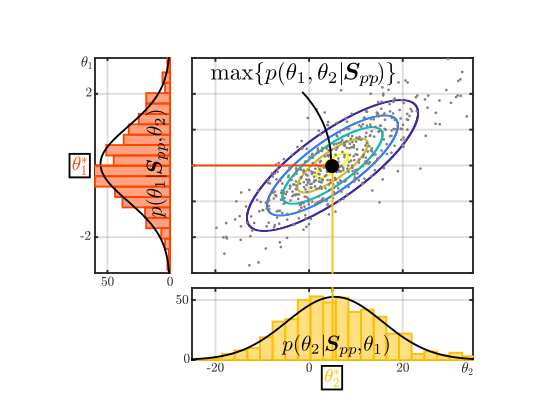
\includegraphics[width=0.8\textwidth]{gibbs.png}\vspace{-0.5ex}
	
\end{minipage}
\hfill
 \begin{minipage}[t]{0.21\textwidth}
		\centering
		\marktikz{step4in} \resizebox{0.5cm}{!}{\circled{\textbf{4}}} \marktikz{step4out} \\[1ex]
		{\bfseries Reconstruire la MI débruitée}\\[1ex]
		\setlength{\fboxsep}{2pt}
		\fcolorbox{black}{vert}{\footnotesize MI mesurée}\\[-0.4ex] = \\[0.5ex]
		\draw[->,line width=1pt ,main,>=latex] (0.5\textwidth-0.1cm,0) -- ++(-1cm,-0.7cm);
		\draw[->,line width=1pt ,main,>=latex] (0.5\textwidth+0.1cm,0) -- ++(1cm,-0.7cm);
		\vspace{0.7cm}
		\noindent ~~ \fcolorbox{black}{jaune}{\footnotesize MI acoustique} \hspace{0.8cm}  \fcolorbox{black}{rouge}{\footnotesize MI bruit}~~~~~~~\\
		\includegraphics[width=0.4\textwidth]{signal.png}  \raisebox{0.15\textwidth}{\large $+$} 
\includegraphics[width=0.4\textwidth]{bruit.png}
\end{minipage}

\tikz[remember picture,overlay]{
	\draw[->,line width=1pt, main,>=latex] ($ (step1out.east)+(0,1ex)$) to [out=20,in=160] ( $ (step2in.west) + (0,1ex) $ );%
	\draw[->,line width=1pt, main,>=latex] ($ (step2out.east)+(0,1ex)$) to [out=20,in=160] ( $ (step3in.west) + (0,1ex) $ );%
	\draw[->,line width=1pt, main,>=latex] ($ (step3out.east)+(0,1ex)$) to [out=20,in=160] ( $ (step4in.west) + (0,1ex) $ );%	
}
 }
 
   \headerbox{}{name=image,span=2,column=4,boxColorOne=gray!12,borderColor=gray!12}{
%  \begin{minipage}[t][1cm][t]{\linewidth}
% 	\centering 	
% 	\noindent \hspace{-3cm}\vspace{2cm}\includegraphics[width=12cm]{contexte.png} 
%\end{minipage}
\begin{minipage}[t][1cm][t]{\textwidth}
	\centering
	\node[inner sep=0pt,overlay,anchor=north west] () at (-1.2cm,1.5cm)  {\includegraphics[width=0.31\paperwidth]{contexte.png} };
\end{minipage}
 }
  
 \headerbox{L'échantillonneur de Gibbs}{name=gibbs,below=methode,column=0,span=3}{
 \noindent $\bullet$ Approxime la distribution jointe inconnue  $p\left(\theta_1,\theta_2,\dots|\bm{S}_{pp}\right)$ \\à partir des distributions conditionnelles connues $p\left(\theta_1|\bm{S}_{pp},\theta_2,\dots\right)$.\\
 \noindent $\bullet$ Méthode de  Monte-Carlo par chaînes de Markov (\textbf{MCMC}) : \\ explore la distribution à l'aide d'une marche aléatoire biaisée.
 
 }

 
 \headerbox{Bruit de fond et des régimes multiples}{name=bf,span=3,column=3 , below=methode}{
 \noindent$\bullet$ On dispose :  \parbox[t][2.4em][t]{0.7\textwidth}{ - d'une mesure de bruit de fond (moteurs coupés),\\
 - de P mesures à différents régimes moteurs.}\\
  \noindent$\bullet$  Hypothèse : même bruit de fond pour les P mesures, à un facteur près.\\
  \noindent$\bullet$ Toutes ces données sont utilisées simultanément pour le débruitage.
 }
 
 \headerbox{Application à l'imagerie}{name=imagerie,column=0,span=6,below=gibbs}{
 \vspace{-2ex}
 \noindent\begin{minipage}{0.65\textwidth}
$\bullet$ Étude du bruit de \textbf{jet supersonique}, not. des cellules de chocs (monopoles corrélés)\\
$\bullet$ Méthode d'\textbf{imagerie} : IRLS avec régularisation bayésienne, forçant la parcimonie des sources
\end{minipage}
\hfill
\begin{minipage}{0.32\textwidth}
\centering
$\bullet$ Erreur de reconstruction : 
\begin{equation*}
\frac{\| \bm{S}_{pp}^{\text{\smaller mesuré}}-\bm{S}_{pp}^{\text{\smaller reconstruit}}\|_1}{\|\bm{S}_{pp}^{\text{\smaller mesuré}}\|_1 \|\bm{S}_{pp}^{\text{\smaller reconstruit}}\|_1} 
\end{equation*}
\end{minipage}
~\\~\\~\\
\centering
\noindent 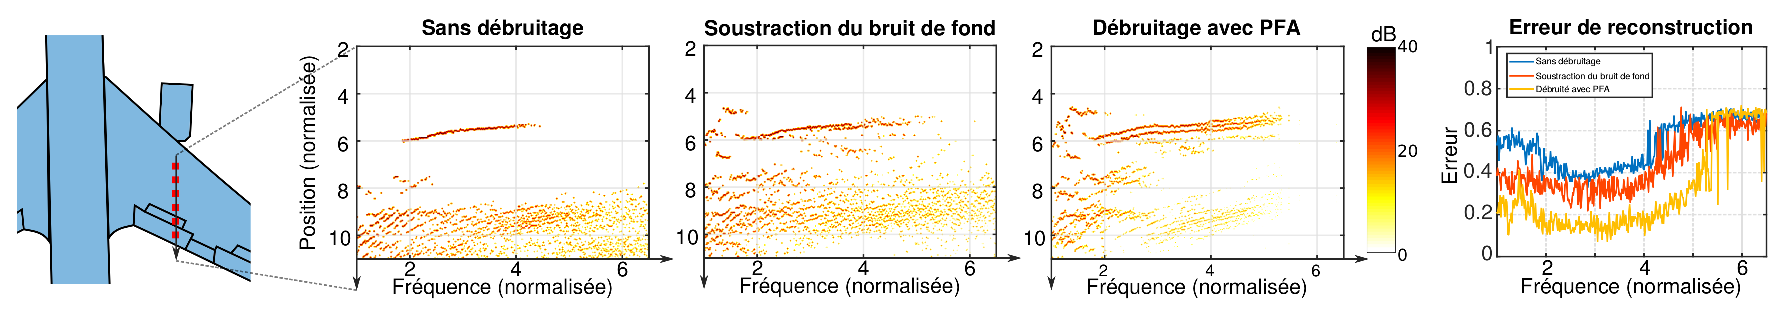
\includegraphics[width=0.9\textwidth]{imagerie_final.eps} 
 
 }
 
 
 \headerbox{Analyse}{name=analyse,column=0, span=4,below=imagerie}{
 \vspace{-1.5em}
  \noindent \hfill \begin{minipage}{0.55\textwidth}
~\centerline{\resizebox{0.5cm}{!}{\circled{\textbf{+}}}} \\[1ex]
 \noindent $\bullet$ MCMC : \parbox[t][2.2em][t]{0.7\textwidth}{  
 - intègre des connaissance \textit{a priori}\\
 - fournit des intervalles de crédibilité}\\~\\
   $\bullet$ PFA : ~~~~ \parbox[t][4.5em][t]{0.8\textwidth}{
  - la MI conserve un sens physique\\
  - réduit la dimension des données\\
- aucun paramètre à régler\\
 - modèle flexible}\\\vfill
\end{minipage}\hfill
\begin{minipage}{0.4\textwidth}
~\centerline{ \resizebox{0.5cm}{!}{\circled{\raisebox{-1ex}{\textbf{-}}}}}\\[1ex]
  - Sensibilité aux choix des \textit{a priori}\\not. si le problème est mal conditionné\\
 -  Coût de calcul élevé\\  \vfill
\end{minipage}
 }
 
 \headerbox{Perspectives}{name=perspective,column=4, span=2,below=imagerie}{
\noindent $\bullet$ Adapter l'échantillonneur pour qu'il soit :\\
- plus robuste (moins sensible aux \textit{a priori}),\\
- plus rapide (meilleure convergence, coût de calcul réduit).\\[0.6ex]
$\bullet$ Adapter le modèle à un bruit corrélé sur les microphones.\\[-1.1ex]
 }
 

 \headerbox{}{name=about,column=0,span=6,below=analyse}{
  	\centering
  	 \footnotesize
	  Contact : \url{alice.dinsenmeyer@insa-lyon.fr}\\
	  \textsuperscript{1}Laboratoire Vibrations Acoustique, Villeurbanne ; 
	\textsuperscript{2}Laboratoire de Mécanique des Fluides et Acoustique, Écully ; 
	\textsuperscript{3}Airbus, Toulouse\\
 	\noindent  \includegraphics[height=1.5cm]{logo/LABEX_CELYA.jpg} \hfill
 	  \includegraphics[trim={0 3cm 0 3cm},clip=true,height=1.5cm]{logo/logo_ADAPT.png} \hfill
 \includegraphics[height=1.5cm]{logo/LVA_compact_couleur.jpg} \hfill
 \includegraphics[height=1.5cm]{logo/logo_lmfa.pdf} \hfill  \\[-3ex]
\hfill \textcolor{gray!50}{\scriptsize  Novembre 2018} \hfill
}

\end{poster}

\end{document}
